\documentclass[UTF8]{ctexart}
\usepackage{dirtree}
\usepackage{listings}
\usepackage{xcolor}
\usepackage{graphicx}
\usepackage{enumerate}
\usepackage[a4paper]{geometry} 
\usepackage{amsmath,amsthm,mathtools}
\usepackage{mathtools}
\usepackage{diagbox}
\usepackage{multirow,makecell}
\usepackage{float}
\usepackage{url}
\usepackage[nottoc]{tocbibind}
\usepackage{float}
\newcommand{\refe}[1]{Eq.\ref{#1}}
\newcommand{\reft}[1]{Theory.\ref{#1}\ }
\newcommand{\reff}[1]{图\ref{#1}\ }
\newtheorem{theorem}{Theory}[section]
\geometry{bottom=2cm,left=1cm,right=1cm}

%插入代码样式设置
\lstset{
 columns=fixed,
 numbers=left,                                        % 在左侧显示行号
 numberstyle=\tiny\color{gray},                       % 设定行号格式
 basicstyle=\small\ttfamily,
 frame=none,                                          % 不显示背景边框
 backgroundcolor=\color[RGB]{245,245,244},            % 设定背景颜色
 keywordstyle=\color[RGB]{40,40,255},                 % 设定关键字颜色
 numberstyle=\footnotesize\color{darkgray},           
 commentstyle=\color{gray}\ttfamily,                  % 设置代码注释的格式
 stringstyle=\rmfamily\slshape\color[RGB]{128,0,0},   % 设置字符串格式
 showstringspaces=false,
 breaklines=true,
 language=python
}

\title{平面最近点对}
\author{张配天-2018202180}
\begin{document}
    \maketitle
    \section{时间复杂度分析}
    由注释,有
    \begin{equation}
        T(n) = \begin{cases}
            \Theta(1)&n\le 4\\
            2T(\frac{n}{2})+O(4n) \implies T(n) = 2T(\frac{n}{2}) + O(n) & n \ge 4\\
        \end{cases}
    \end{equation}
    
    \par 利用代入法,假设$T(n) = O(nlgn)$,对$\forall k < n$有$T(k) \leq cn\lg{n}$,那么
    \begin{gather*}
        T(n) \leq cn(lgn - 1) + 4n = cnlgn - (c-4)n\\
        \implies c-4 \ge 0\implies c \ge 4
    \end{gather*}
    \par 因此,当$c\ge 4$时有$T(n) = O(nlgn)$;
    \par 接下来考虑初始情况,$1*lg1 = 0$,因此取$n_0 \ge 2$,则当$n\ge n_0$时有$T(1) = \Theta(1) \leq cnlgn$,得证。
    \section{空间复杂度分析}
    由于只用一个数组,每一次递归会新建总和比当前数组小的两个数组之后删除,有$O(n)$,而qsort的辅助空间永远为$O(n)$,因此,空间复杂度的为$O(n)$。
    \section{运行截图}
    \begin{figure}[H]
        \centering
        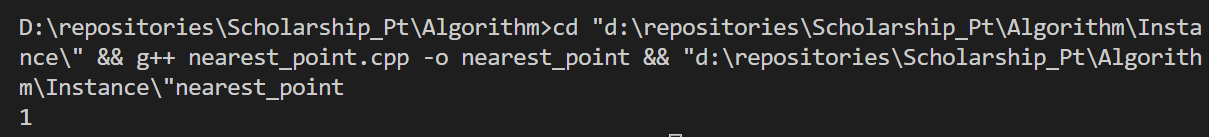
\includegraphics[width=18cm]{../Resources/1.png}
    \end{figure}
    \par 输出最相近点后发现是468,20和468,21。
\end{document}